\documentclass{article}
\usepackage{graphicx}

\begin{document}

\title{ELEC-E7851 - Computational User Interface Design, Assignment 5.1}
\author{Ville Vartiainen}
\date{\parbox{\linewidth}{\centering
  \endgraf
  Student number: 664132}}

\maketitle

\section{Summary of approach}

For the assignment we were supposed to fill in the shoulder torque, strength and endurance variables in the Jupyter notebook. The equations on which they are based could be found in the linked paper on Consumed Endurance. The following equations were found for the variables:
\vspace*{5mm}

Shoulder torque: \hspace{5mm} $\| \overrightarrow{T}_{shoulder} \| = \overrightarrow{r} \cdot m\overrightarrow{g}$
\vspace*{5mm}

Strength: \hspace{5mm} $\frac{\| \overrightarrow{T}_{shoulder} \|}{T_{max}} \cdot 100$
\vspace*{5mm}

Endurance: \hspace{5mm} $E(T_{shoulder}) = \frac{1236.5}{(\frac{T_{shoulder}}{T_{max}} \cdot 100 - 15)^{0.618}}-72.5$
\vspace*{5mm}
\newline

The equations translated into the Jupyter notebook, using the variables already available as the values for the equations:

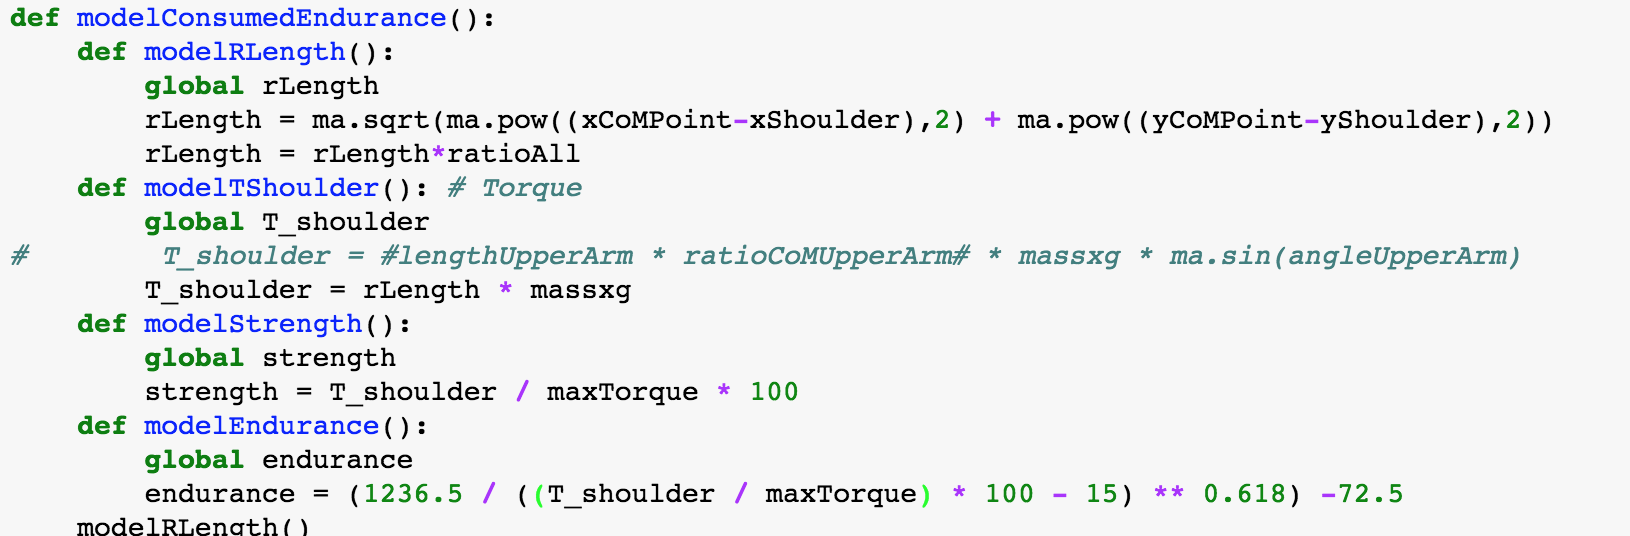
\includegraphics[width=\textwidth,height=\textheight,keepaspectratio]{7-1code}

\section{Screenshots of results}

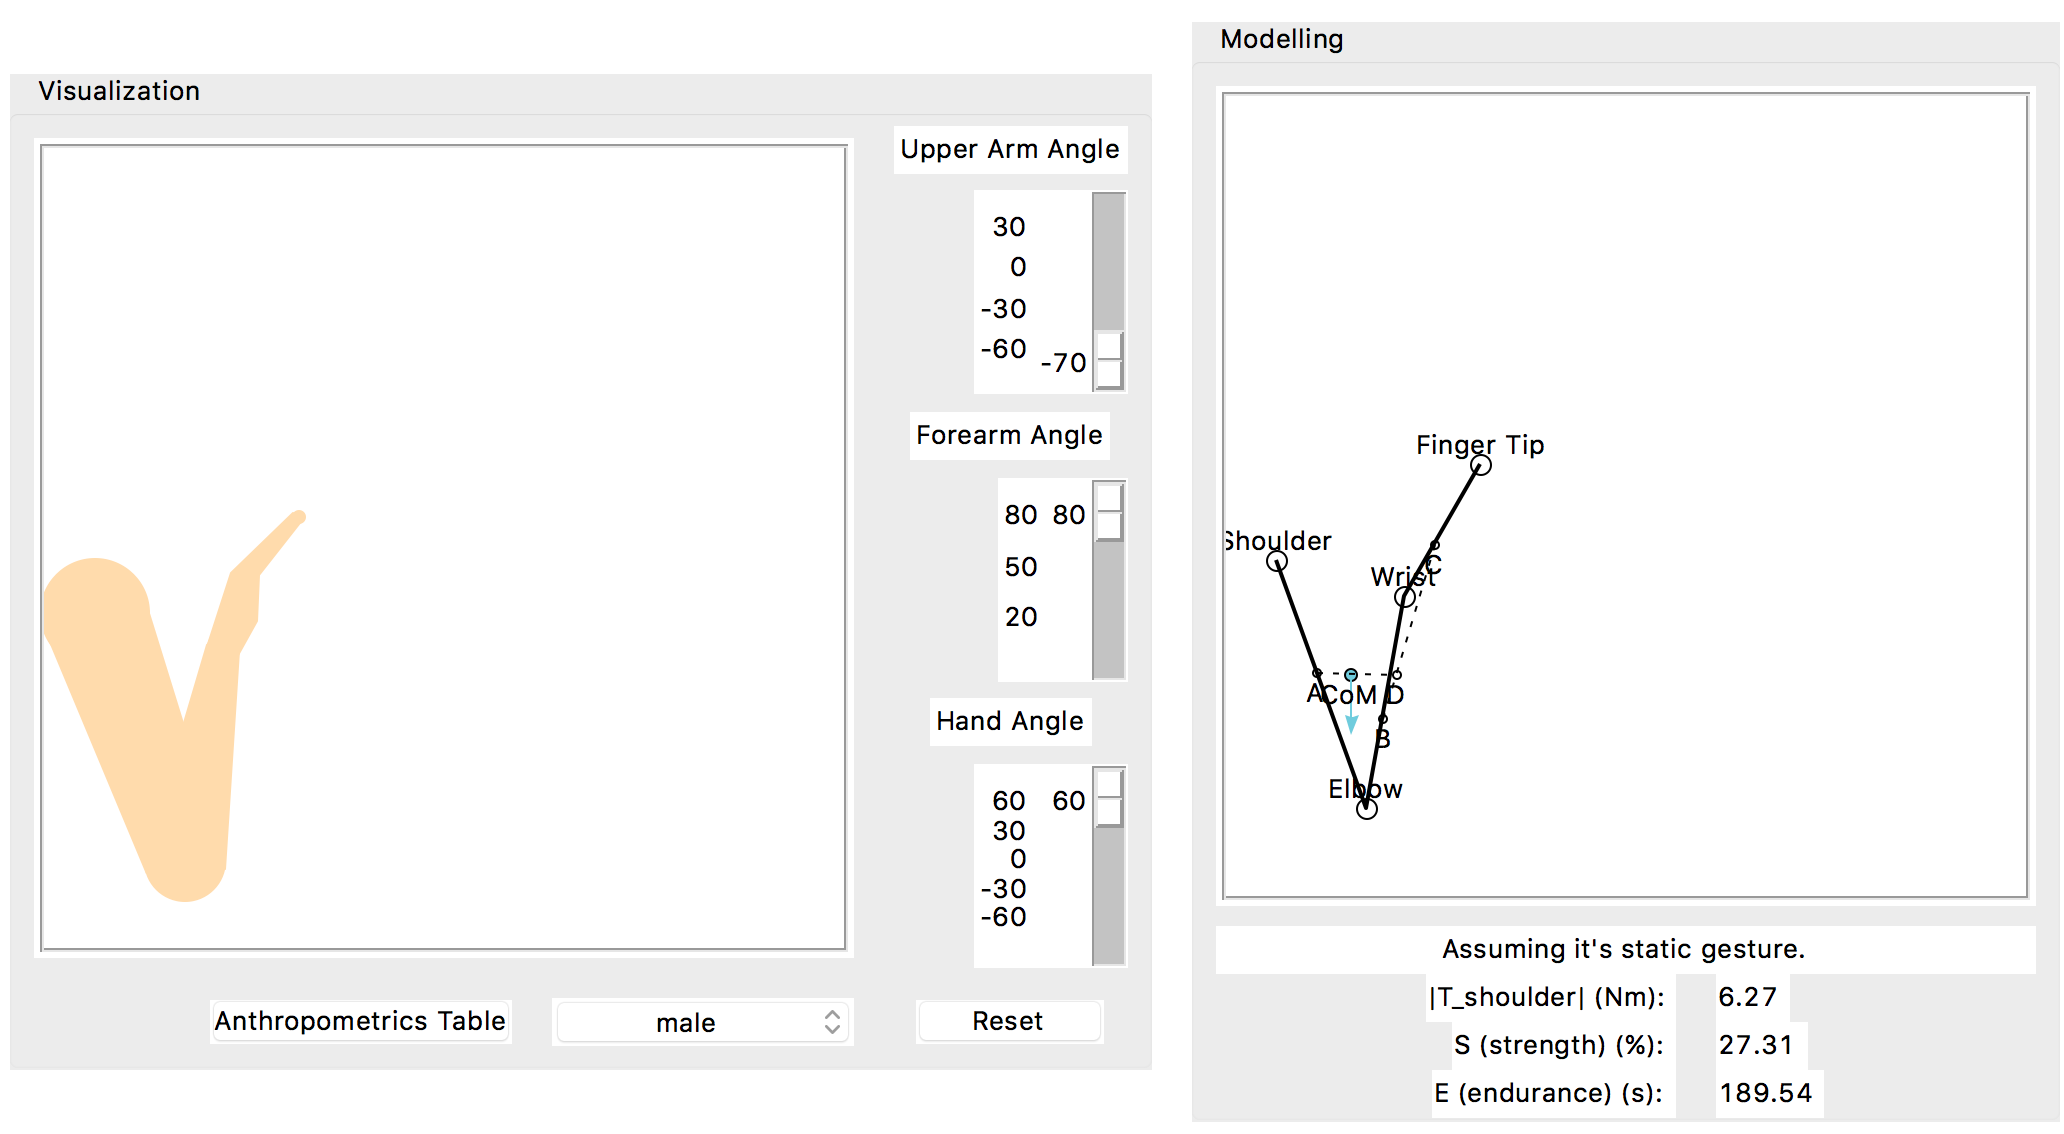
\includegraphics[width=\textwidth,height=\textheight,keepaspectratio]{gui1}\newline
The pose with the highest length of endurance found by adjusting the sliders on the gui looks rather unintuitive and uncomfortable. \vspace*{5mm}\newline
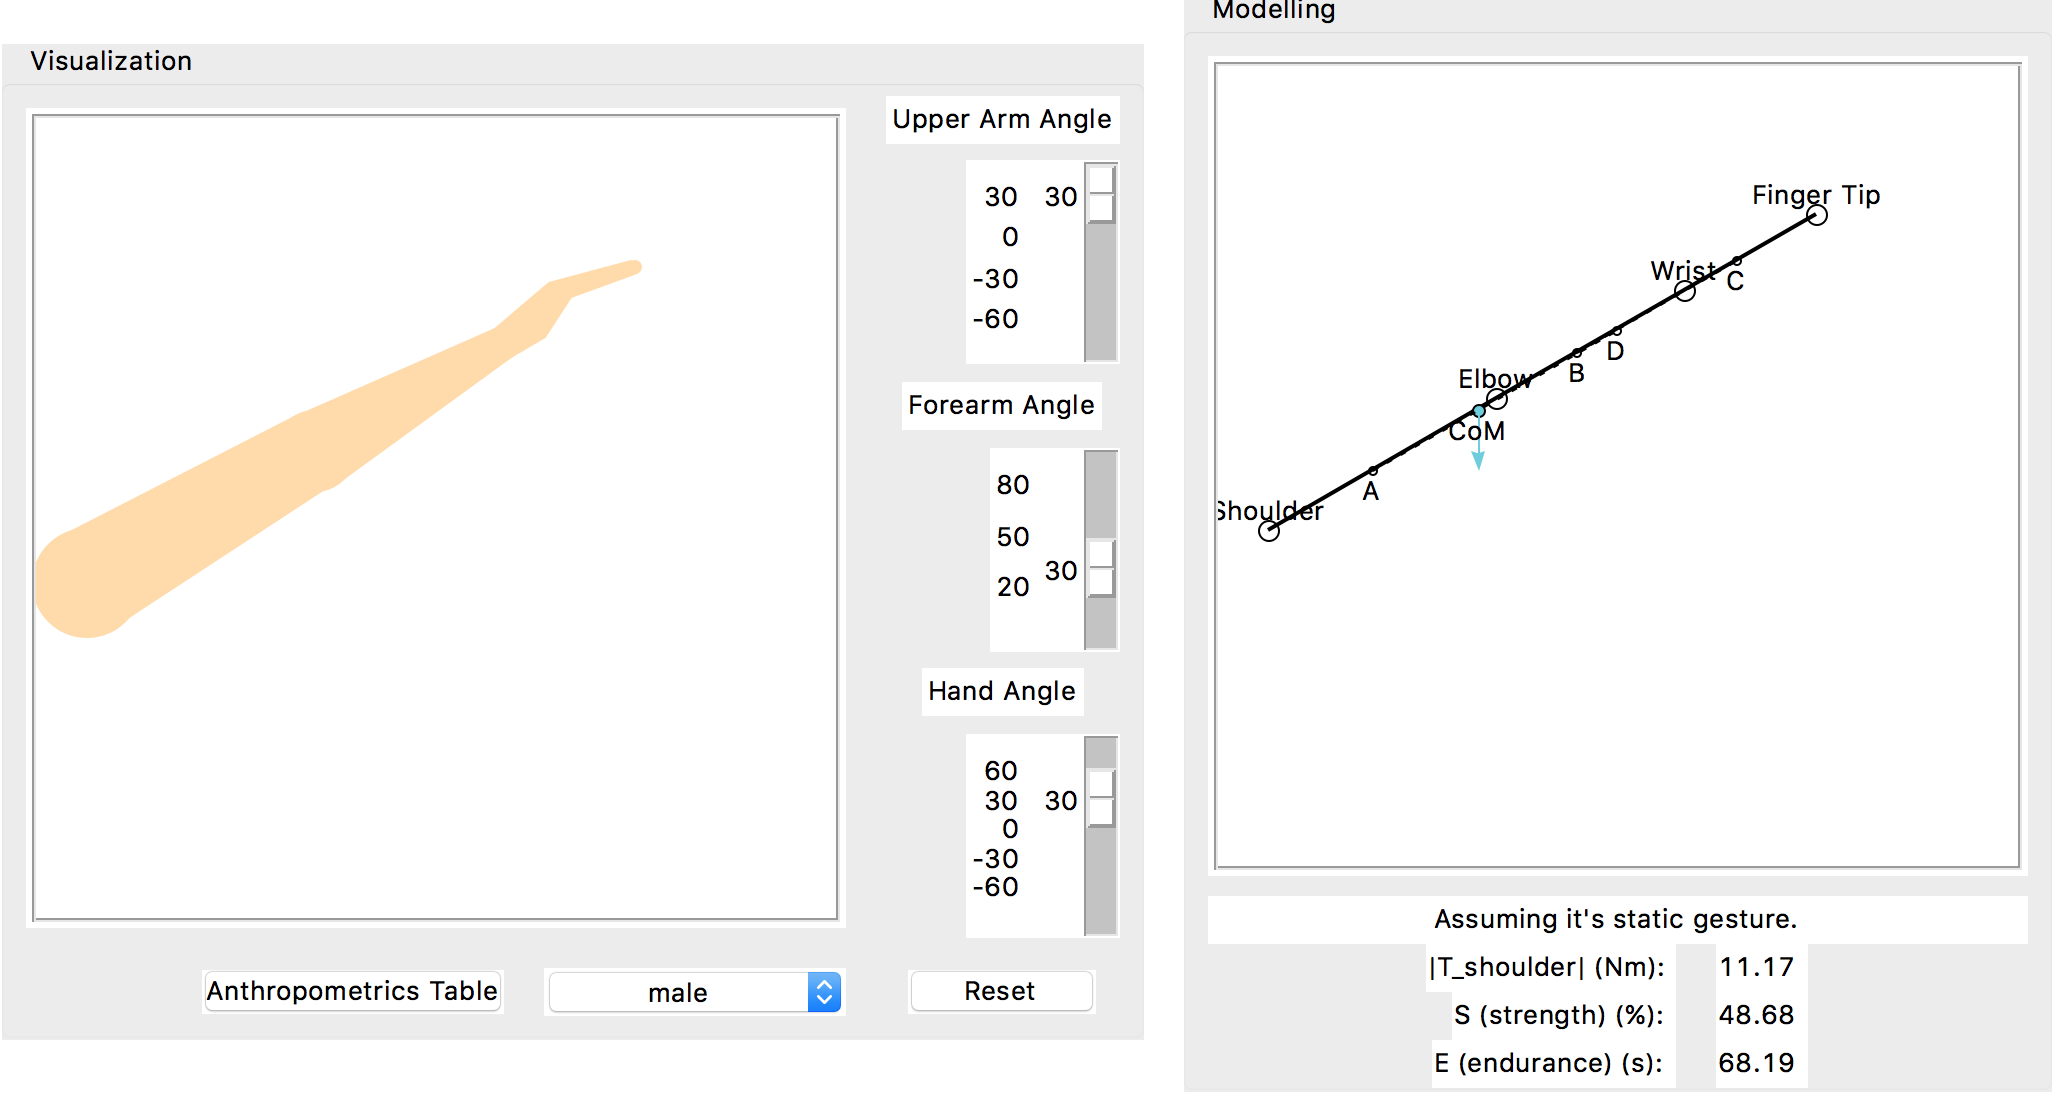
\includegraphics[width=\textwidth,height=\textheight,keepaspectratio]{gui2}\newline
The pose with the shortest endurance has the arm extended and directed slightly upwards.
\vspace*{5mm}
\pagebreak
\section{Evaluation of results}
While I initially had some difficulties with wrapping my head around the formulas, I feel like it all eventually started making relative sense, and that the values displayed by the GUI were at least somewhat making sense - for example the values for endurance seem realistic.

Torque is the rotational force on the shoulder joint, which is why the torque decreases the more the arm is directed directly upwards or downwards. The stronger the torque, the greater the strength required to hold the arm in that particular position, which in the end leads to shortened endurance in positions where the arm is extended horizontally. Strength is the amount of force required to maintain the arm's position. Endurance is the time in seconds the arm can be maintained in a given position.

\end{document}